\chapter{Linear Algebra}
\section{Introduction}
Linear Algebra is all about solving a system of linear equations. It has a general form as shown below.
	\begin{align*}
	a_{11} x_1 + a_{12} x_2  + \cdots + a_{1n} x_n  &= b_1 \\
	a_{21} x_1 + a_{22} x_2  + \cdots + a_{2n} x_n  &= b_2 \\
	& \ \ \vdots\\
	a_{m1} x_1 + a_{m2} x_2  + \cdots + a_{mn} x_n  &= b_ m
	\end{align*}
	
One can interpret this geometrically, where each equation represents a line or a plane or a hyperplane. The \(x\)s can be thought of as the coordinates of the point where the lines or planes or hyperplanes intersect. For example,
	\begin{align*}
	x - y &= -1 \\
	3x+y &= 9
	\end{align*}
represent two lines intersecting in a 2 dimensional space at \((2,3)\) as shown in figure \ref{fig:lines_unique_solution}. \footnote{An alternative geometric interpretation is that x, y are slope and y intercept of a line that contains the coordinates {-1,1} and {3,9} on it. So solving the equations is akin to estimating the (best) line that would transform input values of -1 and 3 to 1 and 9 respectively. Note: One needs to ensure the equations are translated so that they look like mx+c}
	\begin{figure}[h!]
	  \centering
	    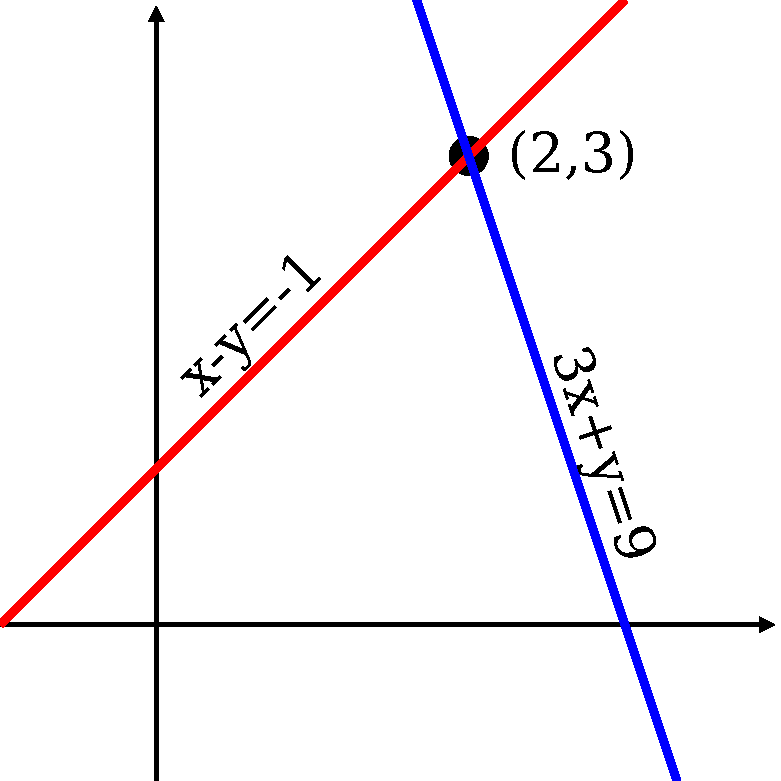
\includegraphics[width=0.25\textwidth]{Linear_Algebra/intersecting_lines}
	  \caption{Intersecting Lines}
	  \label{fig:lines_unique_solution}
	\end{figure}	
Similarly, the equations,
	\begin{align*}
	3x + 2y - z  &= 1 \\
	2x -2y + 4z &= -2 \\
	-x + 0.5y -z &= 0 \\
	\end{align*}
represent three planes intersecting at \((1,-2,-2)\) in a 3 dimensional space as shown in figure \ref{fig:planes_unique_solution} \footnote{Again, we can think of solving for x,y,z as trying to estimate the parameters of a plane that would have transformed a bunch of input values to a bunch of output values (The equations must be translated so that, one of the parameters always has a coefficient of +1). We will deal with this ``geometric dual'' in a later chapter}
	\begin{figure}[h!]
	\centering
	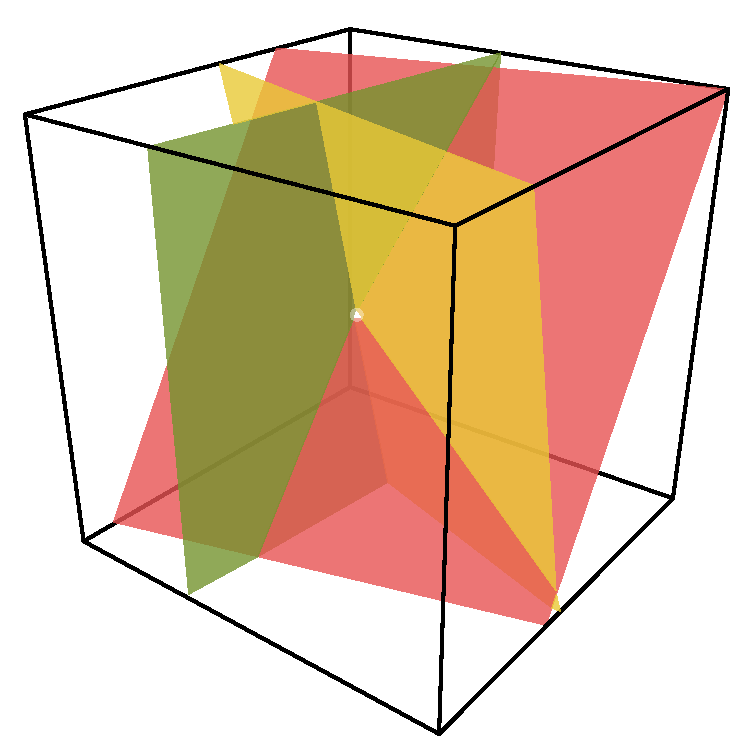
\includegraphics[width=0.25\textwidth]{Linear_Algebra/intersecting_planes}
	\caption{Intersecting Planes}
	\label{fig:planes_unique_solution}
	\end{figure}

With any given system of linear equations, for the unknowns, there could be a unique solution or multiple solutions or no solution at all. Let us look at these possibilities in a 2 dimensional space with two line equations. If the two lines are at different angles, then there is a unique solution. If the two lines are completely overlapping with one another, then there are multiple (infinite) solutions. If the two lines are parallel to each other, then there is no solution. Figure \ref{fig:two_lines} shows these options.
	\begin{figure}[h!]
	\label{fig:Linear_Algebra/two_lines}
	\centering
		\begin{subfigure}{0.3\textwidth}
		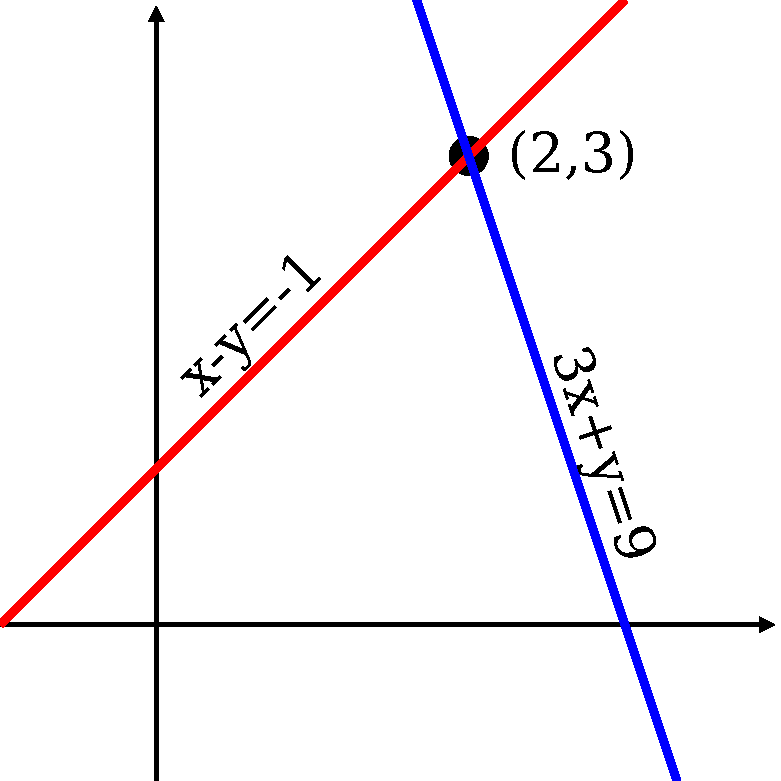
\includegraphics[width=\textwidth]{Linear_Algebra/intersecting_lines}
		\caption{Unique solution}
		\end{subfigure}
		\hspace{1em}
		\begin{subfigure}{0.3\textwidth}
		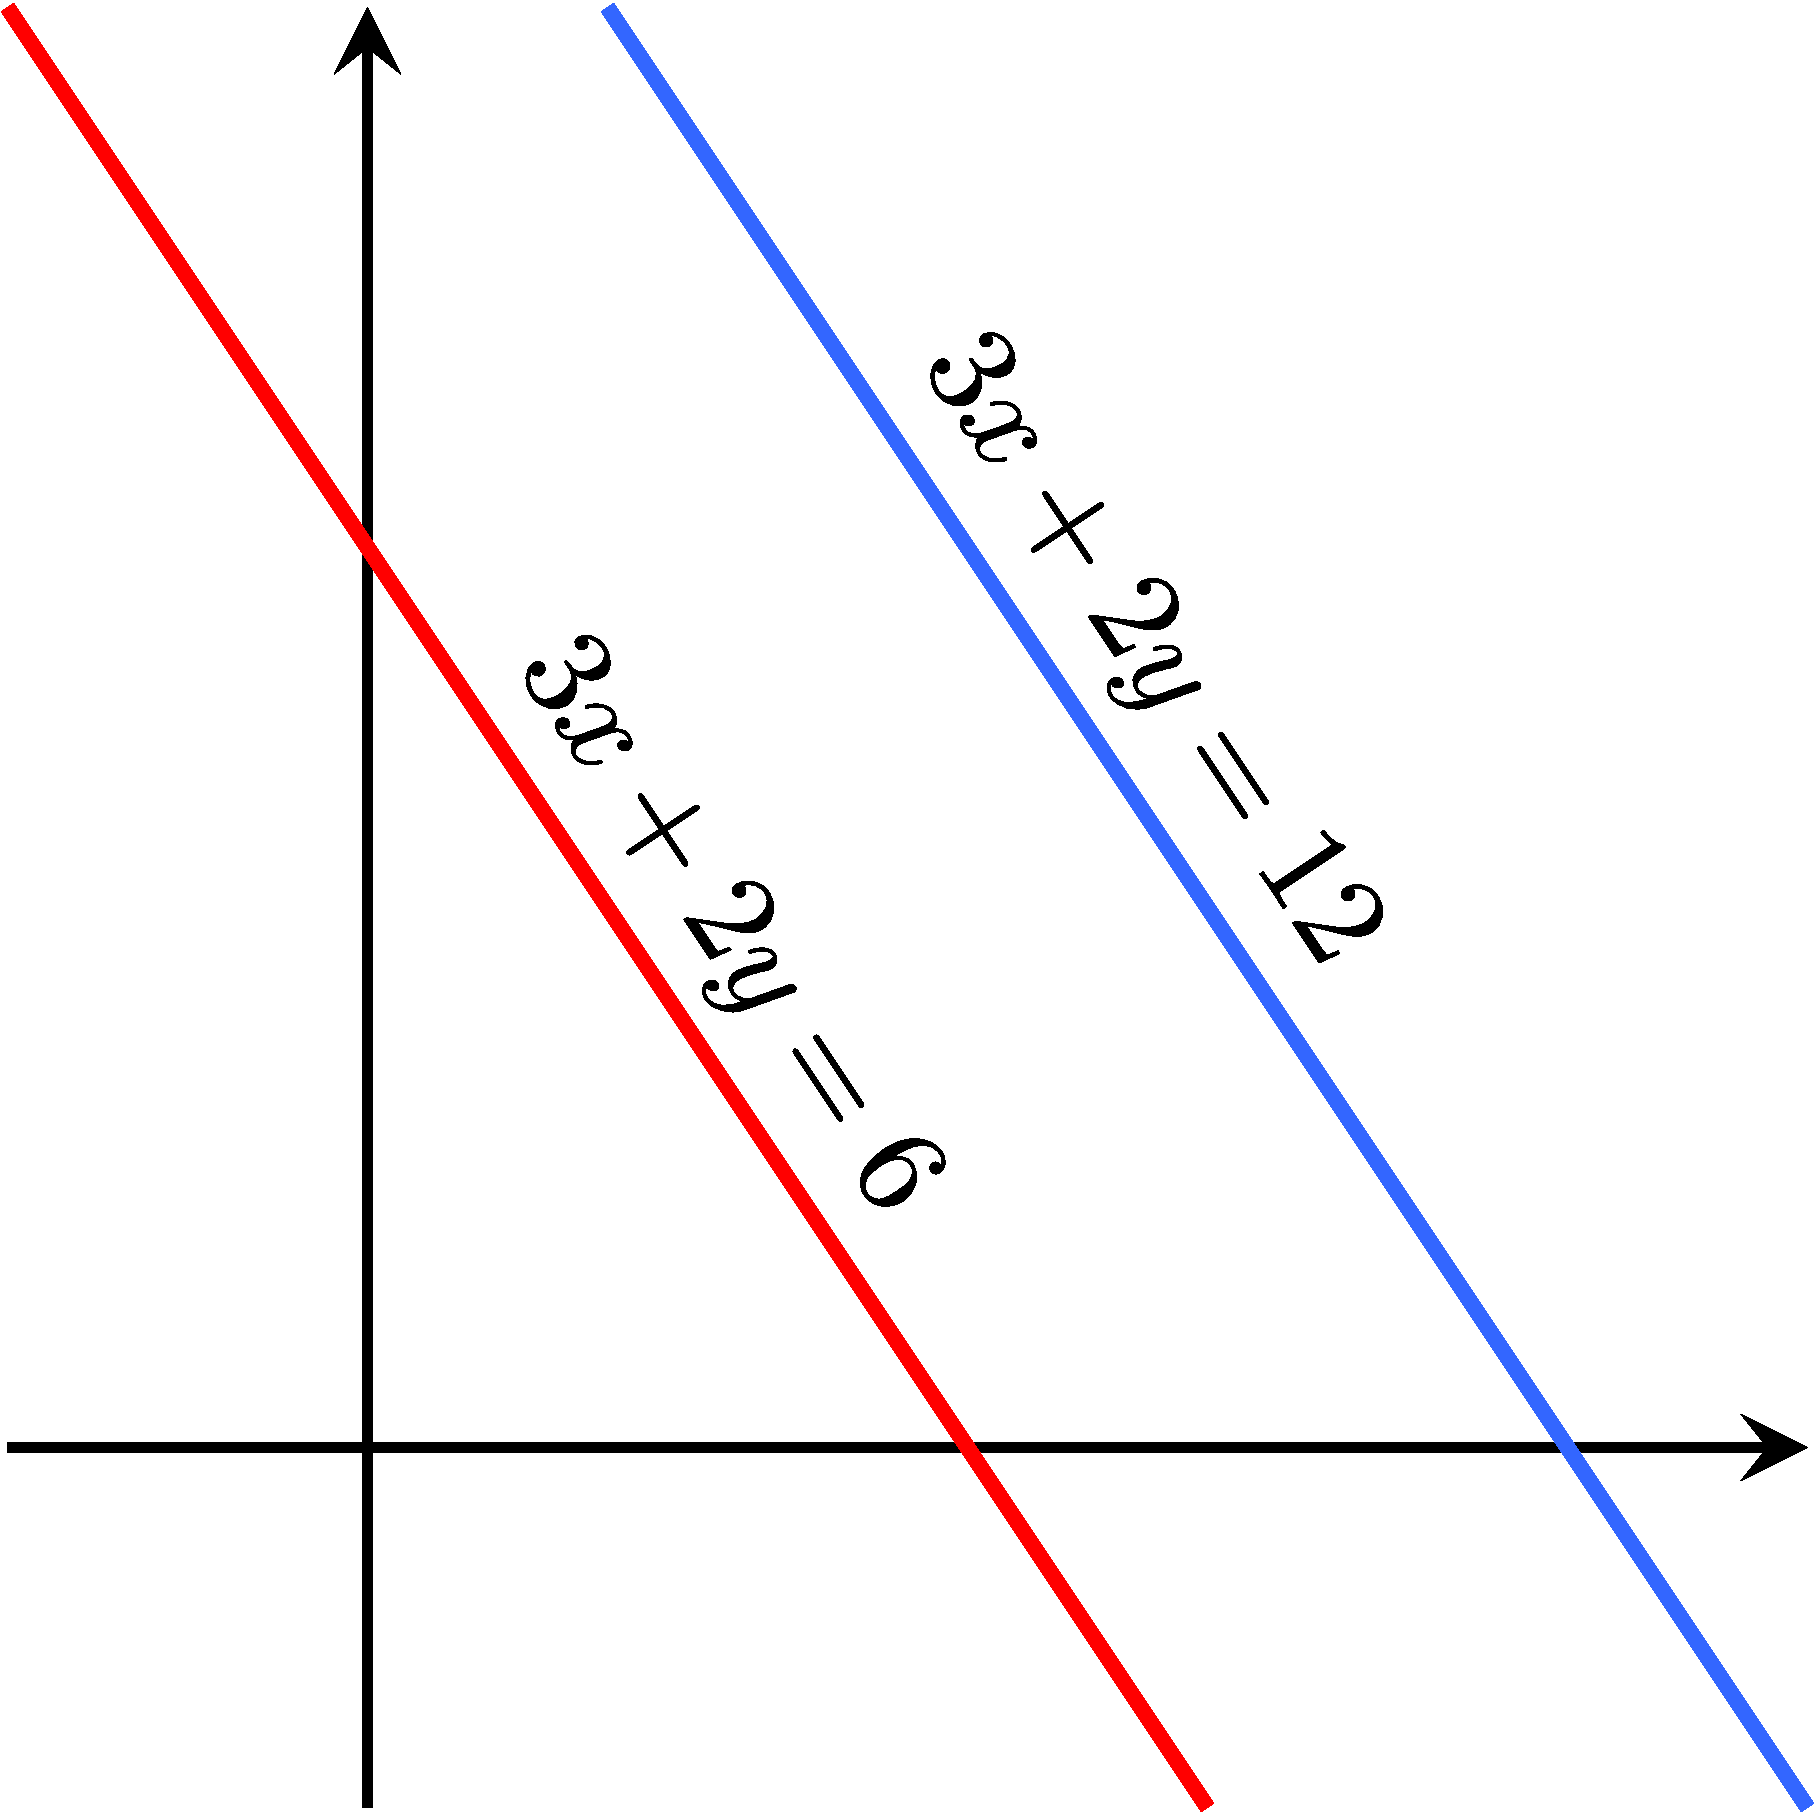
\includegraphics[width=\textwidth]{Linear_Algebra/no_solution}
		\caption{No solution}
		\end{subfigure}
		\hspace{1em}
		\begin{subfigure}{0.3\textwidth}
		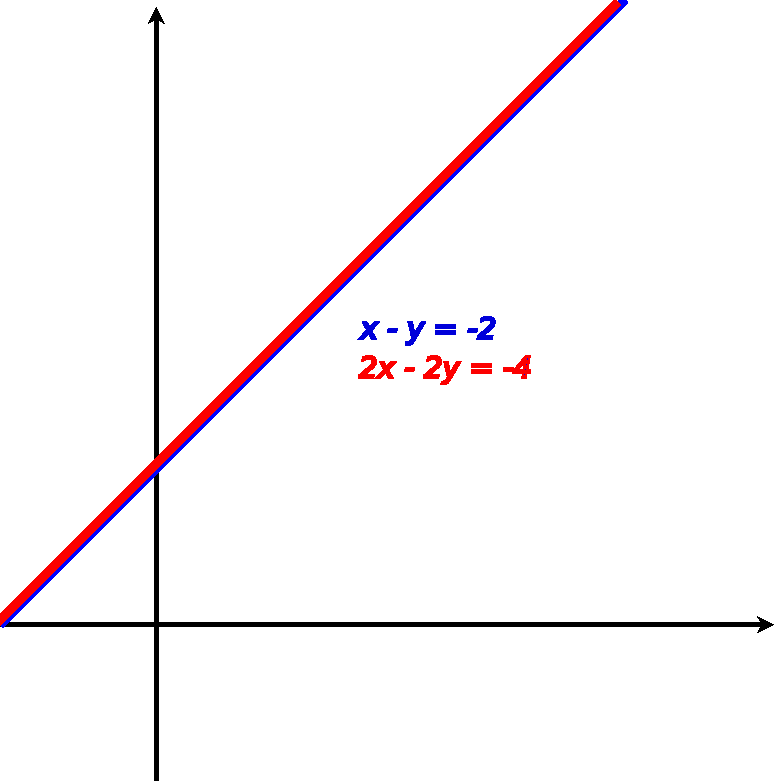
\includegraphics[width=\textwidth]{Linear_Algebra/infinite_solutions}
		\caption{Infinite solutions}
		\end{subfigure}
	\end{figure}

One can notice, that, when two lines overlap and result in infinite solutions, the corresponding equations are linearly related to one another - It is just one information masquerading as two. Linear dependency reduces the number of equations we have and we could end up with less independent equations than we have unknowns. This is called an \textbf{underdetermined system}. The opposite of that - where we have more independent equations than unknown - is called an \textbf{overdetermined system}. An example of an overdetermined system is shown in figure \ref{fig:overdetermined_system}.
	\begin{figure}[h!]
	\centering
	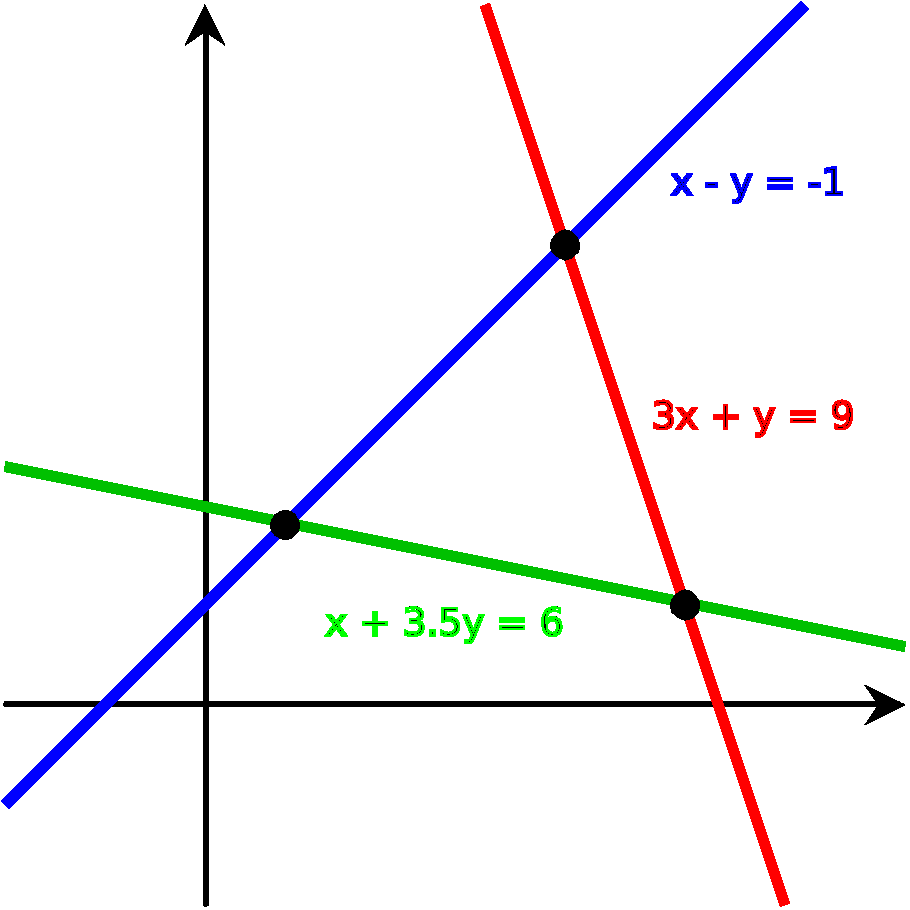
\includegraphics[width=0.25\textwidth]{Linear_Algebra/overdetermined_system}
	\caption{Overdetermined System}
	\label{fig:overdetermined_system}
	\end{figure}
An underdetermined system may have infinite solutions, as we have seen in the overlapping lines example, or no solution - one can think of two parallel planes. An overdetermined system (in general) has no solution. 

We have seen, through a geometric interpretation of lines, a unique solution is possible only if the number of unknowns is the same as the number of independent equations. But when we go beyond lines in 2D space and planes in 3D space, generalizing results, such as what kind of a system results in a unique solution, becomes difficult and non-intuitive (how many can imagine even a 4D space, let alone a much higher dimensional space?). For this, we should go follow a vector spaces approach - The rest of the document deals only with this approach. Vector spaces approach also allows us to go beyond just lines and planes to functions, polynomials etc. 

\section{Vector Spaces Approach}	
This can be written in vector algebra notation as:
	\[ A\mathbf{x}=\mathbf{y} \]
where \(A\) is an \(mxn\) matrix, \(\mathbf{x}\) is a column vector with \(n\) entries, and \(\mathbf{y}\) is a column vector with \(m\) entries.
	\begin{align*}
	A=
	\begin{bmatrix}
	a_{11} & a_{12} & \cdots & a_{1n} \\
	a_{21} & a_{22} & \cdots & a_{2n} \\
	\vdots & \vdots & \ddots & \vdots \\
	a_{m1} & a_{m2} & \cdots & a_{mn}
	\end{bmatrix},\quad
	\mathbf{x}=
	\begin{bmatrix}
	x_1 \\
	x_2 \\
	\vdots \\
	x_n
	\end{bmatrix},\quad
	\mathbf{y}=
	\begin{bmatrix}
	y_1 \\
	y_2 \\
	\vdots \\
	y_m
	\end{bmatrix}
	\end{align*}
One can interpret  \( A\mathbf{x}=\mathbf{y} \) as a linear transformation of \(\mathbf{x}\) vector to \(\mathbf{y}\) by the linear operator \(A\). Or one could think of it as \(\mathbf{y}\) being represented as a linear combination of the columns of \(A\) weighted by rows of \(\mathbf{x}\) as shown below.
	\begin{align*}
		x_1\begin{bmatrix} a_{11}\\ a_{21}\\ \vdots\\ a_{m1} \end{bmatrix} + x_2\begin{bmatrix} a_{12}\\ a_{22}\\ \vdots\\ a_{m2} \end{bmatrix} + \hdots + x_n\begin{bmatrix} a_{1n}\\ a_{2n}\\ \vdots\\ a_{mn} \end{bmatrix}
		= \begin{bmatrix} y_1\\ y_2\\ \vdots\\ y_m \end{bmatrix}
	\end{align*}
In this case, columns of \(A\) can be thought of as vectors themselves. So we could say that we are trying to represent a vector \(\mathbf{y}\) as a linear weighted comination of \(n\) vectors. We will see later that this idea of representing one vector in terms of a set of other vectors has its advantages. But first, we introduce the some important concepts about vector spaces:
	
	\begin{highlightedText}
	\textbf{Definition} A \textbf{linear vector space} \(S\) over a set of scalars \(R\) is a collection of objects known as vectors, together with an additive operation + and a scalar multiplication operation . \footnote{Vector multiplication need not be defined}, that satisfy the following properties
		\begin{itemize}
		\item \(S\) forms a \emph{group} under addition. i.e.,
			\begin{enumerate}
			\item Addition operation is closed.
				\[ \forall \mathbf{x}, \mathbf{y} \in S, \mathbf{x} + \mathbf{y} \in S \]
			\item Identity element, denoted as \(mathbf{0}\) exists, such that
				\[ \mathbf{x} + \mathbf{0} = \mathbf{0}+ \mathbf{x} = \mathbf{x} \]
			\item Additive inverse exists
				\[ \forall \mathbf{x} \in S, \exists \mathbf{y}\ |\ \mathbf{x} + \mathbf{y} = \mathbf{0} \] \footnote{This is just a sneaky way of introducing \(-\) within the definition of the additive operator \(+\).}
			\item Addition is associative
				\[ \forall \mathbf{x}, \mathbf{y}, \mathbf{z} \in S, (\mathbf{x} + \mathbf{y}) + \mathbf{z} = \mathbf{x} + (\mathbf{y} + \mathbf{z}) \]
			\end{enumerate}
		\item \( \forall a, b \in R,\ for\ any\ \mathbf{x}, \mathbf{y} \in S \),
			\begin{enumerate}
			\item \( a\mathbf{x} \in S \)
			\item \( a(b\mathbf{x}) = (ab)\mathbf{x} \)
			\item \( (a + b)\mathbf{x} = a\mathbf{x} + b\mathbf{x} \)
			\item \( a(\mathbf{x} + \mathbf{y}) = a\mathbf{x} + a\mathbf{y} \)
			\end{enumerate}
		\item Multiplicative identity, denoted by \(1 \in R\), exists, such that \(1\mathbf{x} = \mathbf{x}\) 
		\item An element \(0 \in R\) exists, such that \(0\mathbf{x} = \mathbf{0}\) \footnote{Note than multiplicative inverse need not be defined}
		\end{itemize}
	\end{highlightedText}

Before we continue, it is important to understand that the scalars in set \(R\) need not be real or complex numbers as one usually imagines them to be. They can be anything that satisfy operations of additions and multiplications as defined for them. For example, \(R\) can be numbers modulo 256, or even polynomials. Similarly, for vectors, they need not be a collection of real or complex numbers. For example, \(x(t) = c_1 + c_2t + c_3t^2\) can be thought of as a vector \(x(t)\) being represented as a linear combination of vectors \(1, t, t^2\).

Once a vector space is defined with multiplication and addition, one can select a some vectors and linear combination of those will produce numerous vectors in \(S\). 

	\begin{highlightedText}
	\textbf{Definition} If we select a set of vectors \(T \subset S \) then the set of vectors that can be produced by (finite) linear combinations of vectors in T is called the \textbf{span} of T. It is denoted as \(V = span(T)\). \footnote{\(T\) can have infinite number of vectors, but \(V\) will contain only finite linear combinations (which are infinitely many)}
	\end{highlightedText}

Note that \(V\) itself is a vector space! Since \( V \subset S \), \(V\) is called a subspace of \(S\). In other words one could just wildly pick a set of vectors from \(S\) and form a subspace. It can be proved that \(V\) is also the smallest subspace that contains all the vectors in \(T\). Picking a \(T\) and then coming up with a \(V\) is used in some areas like digital communication (out of the scope of this notes), but what about the other way around? If we start with a \(V\) and we want to find a \(T\) whose vectors can span \(V\), we will find several candidates. Then the question arises: ``Which candidate is the best?''. One way to answer it is to find the \(T\) that is the smallest. We will see soon that even in this case we will find several candidates. But let us first focus on what would make a \(T\) the smallest  possible set that spans \(V\). 

Let us take an example \(T1\) that has four vectors namely \( \{ \mathbf{p_1}, \mathbf{p_2}, \mathbf{p_3}, \mathbf{p_4} \} \). Let us take a vector in \(\mathbf{v_1} \in V\). This can be represented as a linear combination of the vectors in \(T1\) as below.
	\[ \mathbf{v_1} = c_1\mathbf{p_1} + c_2\mathbf{p_2} + c_3\mathbf{p_3} + c_4\mathbf{p_4} \].
Now, let us say that \(\mathbf{p4} \) itself can be represented as a linear combination of the remaining three vectors in \(T1\) as:
	\[ \mathbf{p_4} = d_1\mathbf{p_1} + d_2\mathbf{p_2} + d_3\mathbf{p_3} \]
We can substitute this equation in the previous one and get:
	\[\mathbf{ v_1} = (c_1+d_1)\mathbf{p_1} + (c_2+d_2)\mathbf{p_2} + (c_3+d_3)\mathbf{p_3} \]
Since the vector \( \mathbf{v_1} \) is a placeholder for \emph{any} vector in \(V\), this means that the subset \( \{ \mathbf{p_1}, \mathbf{p_2}, \mathbf{p_3} \} \) of \(T1\) itself is a spanning set of \(V\). One could thus come with an initial \(T\) and eliminate vectors in it that can be represented as linear combinations of other vectors and eventually end up with the smallest possible set that can span \(V\). 
	
	\begin{highlightedText}
	\textbf{Definition} A \textbf{Hamel Basis} is a smallest subset of vectors in vector space that can span that vector space.
	\end{highlightedText}

There need not be a unique Hamel Basis for a vector space. But all the Hamel Bases have the following properties.
	\begin{enumerate}
	\item The vectors that comprise a Hamel Basis are linearly independent (of one another), i.e., no vector can be represented as a linear combination of other vectors 
	\item The Hamel Bases all have the same cardinality
	\end{enumerate}
	
We will not go into the proofs of the above points, but they can be found in many text books. So far, we have talked about dimensions casually. But we define it formally now.

	\begin{highlightedText}
	\textbf{Definition} The \textbf{dimension} of a vector space is the cardinality of a Hamel Basis of that vector space. In other words, the dimension of a vector space is the same as the the smallest number of vectors whose linear combination can create any vector in that vector space
	\end{highlightedText}
	
The idea of linear independence at the root of the definition of a Hamel basis is of high importance and hence requires more attention. One way to check if a set of vectors is linearly independent is to see if we can come up with a set of coefficients \( \{c_1, c_2, ...c_n\} \) , not all zeros such that,\( c_1\mathbf{p_1} + c_2\mathbf{p_2} + \ldots + c_n\mathbf{p_n} = \mathbf{0} \), then the vectors\( \{ \mathbf{p_1}, \mathbf{p_2}, \ldots, \mathbf{p_n} \} \) are \emph{not} linearly independent. It is easy to see why: We can readily rewrite \( c_1\mathbf{p_1} + c_2\mathbf{p_2} + \ldots + c_n\mathbf{p_n} = \mathbf{0} \) as:
	\[ c_1\mathbf{p_1} =  (-c_2)\mathbf{p_2} + (-c_3)\mathbf{p_3} + \ldots + (-c_n)\mathbf{p_n} \]
which, by definition, means \(\mathbf{p1}\) is linearly dependent on other \(\mathbf{p}\) vectors. Now, we will use this property to prove that every \( \mathbf{x} \in V \) has a unique representation as a linear combination of vectors in its Hamel basis. To prove this, let us assume that there is an  \( \mathbf{x} \in V \) that can be represented by two different set of coefficients \( \{c_1, c_2, \ldots, c_n\} \) and \( \{d_1, d_2, \ldots, d_n\} \) of the vectors \( \{ \mathbf{p_1}, \mathbf{p_2}, \ldots, \mathbf{p_n} \} \). i.e., 

	\[ c_1\mathbf{p_1} + c_2\mathbf{p_2} + \ldots + c_n\mathbf{p_n} = \mathbf{x} =  d_1\mathbf{p_1} + d_2\mathbf{p_2} + \ldots + d_n\mathbf{p_n} \]
then,
	\[ (c_1-d_1)\mathbf{p_1} + (c_2-d_2)\mathbf{p_2} + \ldots + (c_n-d_n)\mathbf{p_n} = \mathbf{0} \]
Since \( \{ \mathbf{p_1}, \mathbf{p_2}, \ldots, \mathbf{p_n} \} \) are linearly independent, this means that the above equation is only possible if all \( c_i - d_i \) terms are zeroes, or in other words, \( c_i = d_i, \forall i \). Now we can similarly prove that there cannot be two subsets of the Hamel basis, namely \( \{ \mathbf{p_1}, \mathbf{p_2}, \ldots, \mathbf{p_n} \} \), \( \{ \mathbf{q_1}, \mathbf{q_2}, \ldots, \mathbf{q_m} \} \), where \(n\) may or may not be the same as \(m\) and the two sets may or may not have overlaps, i.e, some \(\mathbf{q}\)s same as some \(\mathbf{p}\)s), such that, 
	\[ c_1\mathbf{p_1} + c_2\mathbf{p_2} + \ldots + c_n\mathbf{p_n} = \mathbf{x} =  d_1\mathbf{q_1} + d_2\mathbf{q_2} + \ldots + d_n\mathbf{q_m} \]
then,
	\[ c_1\mathbf{p_1} + c_2\mathbf{p_2} + \ldots + c_n\mathbf{p_n} - d_1\mathbf{q_1} - d_2\mathbf{q_2} - \ldots - d_n\mathbf{q_m} = \mathbf{0} \]
By definition of linear independence, the above equation should only be possible if all the coefficients are \(0\)s, or if the terms with non-zero coefficients all, somehow, cancel each other out. Note that a single term \(c_i\mathbf{p_i}\) or \(d_i\mathbf{q_i}\) itself cannot evaluate to \(\mathbf{0}\) for non-zero coefficient value. So there has to be at least one  \(c_i\mathbf{p_i} - d_i\mathbf{q_i}\), that evaluates to \(\mathbf{0}\), which is only possible, under the assumption of linear independence, if \(c_i = d_i\) and \(\mathbf{p_i} = \mathbf{q_i}\). In other words, 
	\[ c_1\mathbf{p_1} + c_2\mathbf{p_2} + \ldots + c_n\mathbf{p_n} - d_1\mathbf{q_1} - d_2\mathbf{q_2} - \ldots - d_n\mathbf{q_m} = \mathbf{0} \]
implies,
	\begin{itemize}
	\item \(n = m\)
	\item \(c_i = d_i\) 
	\item \(\mathbf{p_i} = \mathbf{q_i}\)
	\end{itemize}
which in turn implies that the representation of \(\mathbf{x}\) as a linear combination of the vectors in the Hamel basis of \(V\) is unique.

With the above concepts in linear algebra, we are almost ready to turn our attention back to solving a system of linear equations: Just one more concept remains as stated in the following Lemma.
	\begin{highlightedText}
	\textbf{Lemma} If we pick any arbitrary set \(B\) of linearly independent vectors that has the same cardinality as the dimension of the vector space \(Y\) of which \(B\) is a subset, then \(B\) is a Hamel basis of \(Y\)
	\end{highlightedText}
The proof is straightforward: Let us assume a condradiction, where there are some vectors in \(Y\) namely, \(\mathbf{y_1}, \mathbf{y_2}, \ldots, \mathbf{y_k}\) that are outside \(span\{B\}\). Then it means that a new set \( B \cup \{ \mathbf{y_1}, \mathbf{y_2}, \ldots, \mathbf{y_k} \} \) will span \(Y\) and hence a Hamel basis of \(Y\). However, this new set's cardinality is greater than that of the dimensionality of the vector space, which is impossible. Hence there cannot be any vector \(\mathbf{y} \in Y\) that is outside \(span\{B\}\). 

Alright, now we are ready to go back to our system of linear equations, \( A\mathbf{x}=\mathbf{y} \), where, 
	\begin{align*}
	A=
	\begin{bmatrix}
	a_{11} & a_{12} & \cdots & a_{1n} \\
	a_{21} & a_{22} & \cdots & a_{2n} \\
	\vdots & \vdots & \ddots & \vdots \\
	a_{m1} & a_{m2} & \cdots & a_{mn}
	\end{bmatrix},\quad
	\mathbf{x}=
	\begin{bmatrix}
	x_1 \\
	x_2 \\
	\vdots \\
	x_n
	\end{bmatrix},\quad
	\mathbf{y}=
	\begin{bmatrix}
	y_1 \\
	y_2 \\
	\vdots \\
	y_m
	\end{bmatrix}
	\end{align*}
If we represent the columns of the matrix \(A\) as \( \mathbf{a_1}, \mathbf{a_1}, \ldots\, \mathbf{a_n} \), then, the system of linear equations boils down to the familiar representation of a vector as a linear combination of other vectors:
	\[ x_1\mathbf{a_1} + x_2\mathbf{a_2} + \ldots + x_n\mathbf{a_n} = \mathbf{y} \]
This is simply an attempt to represent \emph{any} \(\mathbf{y} \in Y\) as a linear combination of some vectors \( \{\mathbf{a_1}, \mathbf{a_2}, \ldots, \mathbf{a_n}\} \).  For a unique solution to exist for this system of linear equations, the following conditions must be true about \( \{\mathbf{a_1}, \mathbf{a_2}, \ldots, \mathbf{a_n}\} \).
	\begin{enumerate}
	\item They must reside in \(Y\)
	\item They should be linearly independent
	\item Their cardinality, \(n\) should be the same as that of any Hamel basis of \(Y\)
	\end{enumerate}
	
To evaluate the first condition, let us look at the concept of \textbf{natural basis} for vectors that are represented as a collection of scalars (as in our case). Any \( \textbf{y} \in Y \) can be represented as:
	\begin{align*}
	\begin{bmatrix}
	y_1 \\
	y_2 \\
	y_3 \\
	\vdots \\
	y_m
	\end{bmatrix} =
	y_1
	\begin{bmatrix}
	1 \\
	0 \\
	0 \\
	\vdots \\
	0
	\end{bmatrix} +
	y_1
	\begin{bmatrix}
	0 \\
	1 \\
	0 \\
	\vdots \\
	0
	\end{bmatrix} + \ldots +
	y_m
	\begin{bmatrix}
	0 \\
	0 \\
	\vdots \\
	0 \\
	1
	\end{bmatrix}
	\end{align*}
	It can be shown that the set \( \{ [1,0,\ldots,0]^T, [0,1,\ldots,0]^T, \ldots, [0,\ldots,0,1]^T \} \) is linearly independent and hence a Hamel basis of \(Y\). With this definition, we can say that any vector \(\mathbf{a}\) resides in \(Y\) as long as it can be represented by the natural basis above. For the vectors \( \{ \mathbf{a_1}, \mathbf{a_2}, \ldots, \mathbf{a_n}\} \), this means that, as long as \(n = m\), they will belong to \(Y\). Note that this also means that \(A\) above has to be a square matrix.

The second condition can be evaluated quite easily using our previous method of finding if there are any set of coefficients that will make the linear combination of \( \mathbf{a_i} \) vectors equal to \(\mathbf{0}\). 

As for the third condition,  \(n = m\), implied by the first condition already ensures that the cardinality of  \( \{ \mathbf{a_1}, \mathbf{a_2}, \ldots, \mathbf{a_n}\} \) is same as that of a Hamel basis (ex. the natural basis). In other words, for a unique solution to exist, all we need is:
	\begin{enumerate}
	\item \(n\) should be the same as \(m\), 
	\item The vectors  \( \{ \mathbf{a_1}, \mathbf{a_2}, \ldots, \mathbf{a_n}\} \) should be linearly independent
	\end{enumerate}
	
But what about the existance of \emph{any} solution at all (whether or not unique)? It can be shown that, if the following conditions are true, a solution and multiple solution will exist.
	\begin{enumerate}
	\item \(n \geq m\), where \(m\) is the cardinality of a Hamel basis of \(Y\)
	\item There are at least \(m\) linearly independent vectors in  \( \{ \mathbf{a_1}, \mathbf{a_2}, \ldots, \mathbf{a_n}\} \)
	\end{enumerate}
To understand these conditions, imagine that \(n = m+1\). When there are at least \(m\) linearly indenpendent vectors in  \( \{ \mathbf{a_1}, \mathbf{a_2}, \ldots, \mathbf{a_n}\} \), we have:
	\[ \mathbf{a_n} = c_1\mathbf{a_1} + c_2\mathbf{a_2} + \ldots + c_m\mathbf{a_m} \]
Now, using this we can show the following:
	\[ \mathbf{y} = x_1\mathbf{a_1} + x_2\mathbf{a_2} + \ldots + x_n\mathbf{a_n} \]
	\[ \mathbf{y} = x_1\mathbf{a_1} + x_2\mathbf{a_2} + \ldots + x_m\mathbf{a_m} + c_1\mathbf{a_1} + c_2\mathbf{a_2} + \ldots + c_m\mathbf{a_m} \]
	\[ \mathbf{y} = (x_1 + c_1)\mathbf{a_1} + (x_2 + c_2)\mathbf{a_2} + \ldots + (x_2 + c_m)\mathbf{a_m} \]
Since \( \{ \mathbf{a_1}, \mathbf{a_2}, \ldots, \mathbf{a_n}\} \) is a Hamel basis of \(Y\), this means that one can find unique coefficents, say, \( \{k_1, k_2, \ldots, k_m \} \) that satisfy the above equation, where, 
	\[ k_i = x_i + c_i, \forall i \in [1,m] \]
So, whereas we can find unique \(k_i\)s, and hence at least one solution for \(x_i\)s  exists, multiple possible values of \(c_i\)s and \(x_i\)s exists, that will give these \(k_i\)s - So we have indeed multiple solutions for \(x_i\)s (i.e., we have multiple solutions for the linear system of equations). One can see that, when multiple solutions exist, \(n > m\) makes the system of equations an \textbf{underdetermined} one.

Needless to say, if the conditions for the existance of at least one solution are not satisfied, then no solution would exist. For ex., if the number of linearly independent vectors in \( \{ \mathbf{a_1}, \mathbf{a_2}, \ldots, \mathbf{a_n}\} \) is less than m: say, m-1, then, \( \{ \mathbf{a_1}, \mathbf{a_2}, \ldots, \mathbf{a_n}\} \) will span a space that is one dimension smaller than \(Y\), i.e, they will span a subspace of \(Y\). In that case, there is a way of finding the vector \( \hat{\mathbf{y}} \) in this subspace of \(Y\) that is closest to \(\mathbf{y}\). This is called an approximation problem \footnote{where we have (possibly with some manipulations) an \textbf{overdetermined} system of equations. }. Exploring this approximation problem requires that we define some measure of length of a vector (called, ``norm'') and a measure of projection of one vector over another (called, ``inner product''). 

\subsection{Norm and inner product}

	\begin{highlightedText}
	\textbf{Definition} A real valued function of a vector \(\mathbf{x} \in S\), denoted as \inorm{x}.is said to be a \textbf{norm} if \inorm{x} satisfies the following properties.
	\begin{enumerate}
	\item \( \|x\| \geq 0 \ \forall\  \mathbf{x} \in S \) 
	\item \inorm{x} = 0 if and only if \ivec{x} = 0
	\item \( \| \alpha \mathbf{x} \| = |\alpha| \  \|\mathbf{x}\| \), where \(\alpha\) is an arbitrary scalar
	\item \( \| \mathbf{x} + \mathbf{y} \| \leq \| \mathbf{x} \| + \| \mathbf{y} \| \). This is called triangule inequality.
	\end{enumerate}
	if \inorm{x} is a norm then \( d(\mathbf{x},\mathbf{y}) = \| \mathbf{x} - \mathbf{y} \| \) is a metric. 
	\end{highlightedText}
	
	The point about the norm being used as a metric is intuitive: one can think of \inorm{x} as \(d(\mathbf{x},\mathbf{0})\). And the distance between a vector \ivec{y} and its approximation, \ivec{\hat{y}} can be thought of as the length of the approximation ``error vector'' \ivec{e}, i.e., \( \| \mathbf{e} \| = d(\mathbf{y} - \hat{\mathbf{y}}) = \| \mathbf{y} - \hat{\mathbf{y}} \| \). 
	
	The most popular norms are (\(n\) is the dimension of the vector):
	\begin{enumerate}
	\item The \(l_1\) norm: \( \| \mathbf{x} \|_1 = \sum_{i=1}^{n} |x_i| \)
	\item The \(l_p\) norm: \( \| \mathbf{x} \|_p = (\sum_{i=1}^{n} |x_i|^p)^{1/p} \)
	\item The \(l_\infty\) norm: \( \| \mathbf{x} \|_\infty = max_{i = 1, 2, \ldots, n} |x_i| \)
	\end{enumerate}

The \(l_2\) norm of the ``error vector'' is basically the Euclidean distance between \ivec{y} and \ivechat{y}. Note that, although the exact values of a norm will differ from one definition of the norm to another, a vector that is small with respect to one norm is also small with respect to another norm. 

	\begin{highlightedText}
	\textbf{Definition} An \textbf{inner product} in a vector space \(S\) is a function that operates on two vectors and returns a scalar, i.e., \( \inp{\cdot} {\cdot}:\ S \times S \rightarrow R\). It has the following properties:
	\begin{enumerate}
	\item \( \inpb{x}{y} = \inpb{y^*}{x^*}\)
	\item \( \inp{\alpha \mathbf{x}}{\mathbf{y}} = \alpha \inpb{x}{y} \)
	\item \( \inpb{x+y}{z} = \inpb{x}{z} + \inpb{y}{z} \)
	\item \( \inpb{x}{x} > 0 \) if \( x \neq 0 \), and \( \inpb{x}{x} = 0 \), if and only if, \( \mathbf{x} = \mathbf{0} \) 
	\end{enumerate}
	\end{highlightedText}

The most popular inner product is \( \inpb{x}{y} = \mathbf{y}^H \mathbf{x} \) (For real vectors, the hermitian becomes just a transpose). One can define a norm in terms of the inner product. Such a norm is called an \textbf{induced norm}. For example, we can defined the \(l_2\) norm as \( \normb{x} = {\inpb{x}{x}}^{1/2} \). 

One can geometrically interpret the inner product as a function of the angle between two vectors. If one were to represent the two vectors using polar coordinates as \( \mathbf{x} = [r_1 cos\theta_1, r_1 sin\theta_1] \) and \( \mathbf{y} = [r_2 cos\theta_2, r_2 sin\theta_2] \), then if we compute the inner product \( \mathbf{y^Tx} \), it will result in \(r_1 r_2 cos(\theta_1 - \theta_2)\). Also the induced norms of \ivec{x} and \ivec{y} will end up as \(r_1\) and \(r_2\) respectively. So one can infer that, 
	\[ cos(\theta_1 - \theta_2) = \frac{\inpb{x}{y}}{\normb{x}\normb{y}} \]
Although we have used \(\mathbb{R}^2\) in this example, one can extend this geometric interpretation to higher dimensions, because, when we are considering two vectors, we can always come up with a 2D subspace in which both vectors reside and then the maths will follow. 

An important implication of this geometric interpretation is that, if two vectors are perpendicular to each other, then their inner product is \(0\) \marginnote{In fact, in a normed vector space, no matter how the norm is defined, two vectors in that space are said to be orthogonal if their inner product is \(0\). So even when the vectors are functions or polynomials, and the inner product has integrals and what not, the idea of orthogonality can be extended using this definition}. This fact is very useful for our next geometric interpration of the inner product: inner product as a projection of one vector on another. Check out figure \ref{fig:inner_product_projection}. 
	\begin{figure}[h!]
	\centering
	\includegraphics[width=0.5\textwidth]{Linear_Algebra/inner_product_projection}
	\caption{Inner product as a projection}
	\label{fig:inner_product_projection}
	\end{figure}
We show two vectors \ivec{y} and \ivec{a}. One can imagine \ivec{a} being parallel to the ground (if you will). Now imagine the sun at 12`O' clock. It will create a shadow of \ivec{y} on \ivec{a}. Let us call the length of this shadow as \(x\). Now one can imagine a third vector \ivec{e} connecting the end of the shadow to the end of \ivec{y}. We can show that,
	\begin{align*}
	\mathbf{y} &= x\mathbf{a} + \mathbf{e} \\
	\inpb{y}{a} &= x^2\inpb{a}{a} + \inpb{e}{a}
	\end{align*}
	Now, using our previous understanding of inner product of two vectors orthogonal to each other being \(0\)
	\[ \inpb{y}{a} = x^2\normb{a}^2 + 0 \]
	If \ivec{a} is a unit vector, then,
	\[ \inpb{y}{a} = x^2 \] 
In other words, if \ivec{a} is a unit vector, then the inner product \( \inpb{y}{a} \) is square of the length of the shadow of \ivec{y} falling on \ivec{a}.
	
Now, recall our linear system of equations, represented as 
	\[  \mathbf{y} = x_1\mathbf{a_1} + x_2\mathbf{a_2} + \ldots + x_n\mathbf{a_n} \]
One can generate an alternative system of linear equations by calculating the norm of \ivec{y} with each of the \ivec{a_i} as shown below:
	\begin{align*}
	\inpb{y}{a_1} &= x_1\inpb{a_1}{a_1} + x_2\inpb{a_2}{a_1} + \ldots + x_n\inpb{a_n}{a_1} \\ 
	\inpb{y}{a_2} &= x_1\inpb{a_1}{a_2} + x_2\inpb{a_2}{a_2} + \ldots + x_n\inpb{a_n}{a_2} \\
	\vdots \\
	\inpb{y}{a_n} &= x_1\inpb{a_1}{a_n} + x_2\inpb{a_2}{a_n} + \ldots + x_n\inpb{a_n}{a_n} \\
	\end{align*}
In matrix notation, we can represent this as:
	\[ R\mathbf{x} = \mathbf{p} \]
where,
	\begin{align*}
	R=
	\begin{bmatrix}
	\inpb{a_1}{a_1} & \inpb{a_2}{a_1} & \cdots & \inpb{a_n}{a_1} \\
	\inpb{a_1}{a_2} & \inpb{a_2}{a_2} & \cdots & \inpb{a_n}{a_2} \\
	\vdots & \vdots & \ddots & \vdots \\
	\inpb{a_1}{a_n} & \inpb{a_2}{a_n} & \cdots & \inpb{a_n}{a_n} \\
	\end{bmatrix},\quad
	\mathbf{x}=
	\begin{bmatrix}
	x_1 \\
	x_2 \\
	\vdots \\
	x_n
	\end{bmatrix},\quad
	\mathbf{p}=
	\begin{bmatrix}
	\inpb{y}{a_1} \\
	\inpb{y}{a_2} \\
	\vdots \\
	\inpb{y}{a_n}
	\end{bmatrix}
	\end{align*}

So, one could use \(\mathbf{x} = R^{-1}\mathbf{p}\) as much as \(\mathbf{x} = A^{-1}\mathbf{y}\). It turns out that, just as we found out that \(A^{-1}\) would exist only if \ivec{a_i} are linearly independent, the same is true for the existence of the \(R^{-1}\). The matrix \(R\) is called the \textbf{Grammian matrix}. The Grammian matrix is always a square matrix and hermitian symmetric, i.e., \(R^H = R\). 

There are three advantages of using \(\mathbf{x} = R^{-1}\mathbf{p}\) over \(\mathbf{x} = A^{-1}\mathbf{y}\):
	\begin{enumerate}
	\item \(R\) is always a matrix whether or not \(A\) is a matrix (Recall the note about how a vector need not a tuple of scalars...how a function or a polynomial can be a vector)
	\item When it comes to finding a solution for overdetermined system of equations where no solutions exist, the former method can be used with some tricks. We explain this in the next section.
	\item Because \(R\) is hermitian symmetric, it is easier to invert than \(A\) that, in general, has no structure.    
	\end{enumerate}
Before we move on, we make a note about the relationship between these two equivalent solutions. One can easily see that \(R\) is nothing but \(A^H A\), and \(\mathbf{p}\) is nothing but \(A^H \mathbf{y}\). So one can rewrite \(\mathbf{x} = R^{-1}\mathbf{p}\) as:
	\[ \mathbf{x} = (A^H A)^{-1} A^H \mathbf{y} \]
The usefulness of the above representation will be more apparent in the next section.

\section{Approximation}
In the previous chapter, we saw the conditions for the existence of a unique solution to \(A\mathbf{x} = \mathbf{y}\), and for the existence of at least once (and many) solutions to the same. In this chapter we focus on the an overdetermined system of equations where no solutions exist. Below is such a system of equations:
	\begin{align*}
		x_1\begin{bmatrix} a_{11}\\ a_{21}\\ \vdots\\ a_{m1} \end{bmatrix} + x_2\begin{bmatrix} a_{12}\\ a_{22}\\ \vdots\\ a_{m2} \end{bmatrix} + \hdots + x_n\begin{bmatrix} a_{1n}\\ a_{2n}\\ \vdots\\ a_{mn} \end{bmatrix}
		= \begin{bmatrix} y_1\\ y_2\\ \vdots\\ y_m \end{bmatrix}
	\end{align*}
We saw in the previous chapter that a system is overdetermined if \(n<m\). When there exists no solution to \ivec{x}, one can find the best candidate for \ivec{x} that will result in a \ivechat{y} that is closest to \ivec{y}. It turns out that this best candidate will be unique. Let us see how this happens by first representing this concept mathematically as:
	\[ \mathbf{y} = \hat{\mathbf{y}} + \mathbf{e} \]
If we were to visualize this relationship, it is intuitive that we can minimize ivec{e} when \ivec{e} is orthogonal to \ivechat{y}. This is shown in figure \ref{fig:orthogonal_error}
	\begin{figure}[h!]
	\centering
	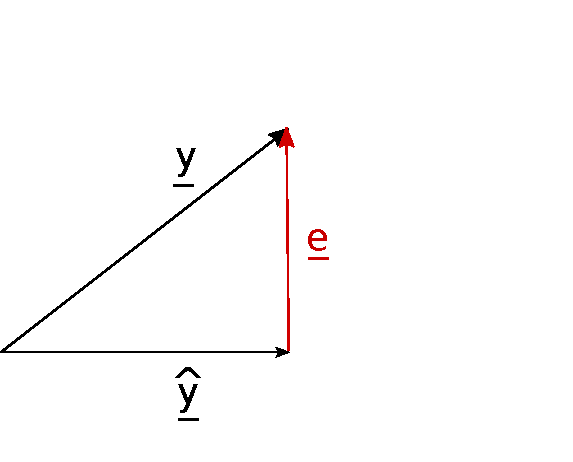
\includegraphics[width=0.5\textwidth]{Linear_Algebra/orthogonal_error}
	\caption{Minimum error}
	\label{fig:orthogonal_error}
	\end{figure}	
Substituting \ivechat{y} in terms of \ivec{x}, we get,
	\[ \hat{\mathbf{y}} = x_1\mathbf{a_1} + x_2\mathbf{a_2} + \ldots + x_n\mathbf{a_n} \]
In other words,
	\[ \mathbf{y} = x_1\mathbf{a_1} + x_2\mathbf{a_2} + \ldots + x_n\mathbf{a_n} + \mathbf{e} \]
Taking the inner product of \ivec{y} with every \ivec{a_i}, we establish our familiar alternative system of linear equations:
	\begin{align*}
	\inpb{y}{a_1} &= x_1\inpb{a_1}{a_1} + x_2\inpb{a_2}{a_1} + \ldots + x_n\inpb{a_n}{a_1} + \inpb{e}{a_1}\\ 
	\inpb{y}{a_2} &= x_1\inpb{a_1}{a_2} + x_2\inpb{a_2}{a_2} + \ldots + x_n\inpb{a_n}{a_2} + \inpb{e}{a_1}\\
	\vdots \\
	\inpb{y}{a_n} &= x_1\inpb{a_1}{a_n} + x_2\inpb{a_2}{a_n} + \ldots + x_n\inpb{a_n}{a_n} + \inpb{e}{a_1}\\
	\end{align*}
If \ivec{e} minimized when it is orthogonal to \ivechat{y}, it will be orthogonal to every \ivec{a_i}. So this system of equations becomes:
	\begin{align*}
	\inpb{y}{a_1} &= x_1\inpb{a_1}{a_1} + x_2\inpb{a_2}{a_1} + \ldots + x_n\inpb{a_n}{a_1} \\ 
	\inpb{y}{a_2} &= x_1\inpb{a_1}{a_2} + x_2\inpb{a_2}{a_2} + \ldots + x_n\inpb{a_n}{a_2} \\
	\vdots \\
	\inpb{y}{a_n} &= x_1\inpb{a_1}{a_n} + x_2\inpb{a_2}{a_n} + \ldots + x_n\inpb{a_n}{a_n} \\
	\end{align*}
And this is exactly the same as the alternative system of equations \( R\mathbf{x} = \mathbf{p} \) we obtained in the previous chapter for solving \ivec{x}, when \ivec{a_i} are linearly independent! So the solution \(\mathbf{x} = R^{-1}\mathbf{p}\) for finding the unique solution for \ivec{x} also works for finding the best solution for \ivec{x} when \ivec{y} isn't reachable by \ivec{x}! As before we can write the solution entirely in terms of \(A\) as:
	\[ \mathbf{x} = (A^H A)^{-1} A^H \mathbf{y} \]
This is called the \textbf{least squares solution}. Compare this equation to \(\mathbf{x} = A^{-1}y\), which will work only in the specfic case of \(n = m\). the above equation will work for the general case of \(n \leq m\) as long as \ivec{a_i} are linearly independent. Hence, \((A^H A)^{-1} A^H\) is called a \textbf{pseudo inverse} of \(A\). So, in the case of a properly-determined system, the pseudo inverse based solution works out to be the same as that of the regular inverse, in the case of an over-determined system of equations This also means that, in the case of linearly \emph{dependent} set of equations, while multiple solutions exists, one way to find a solution is to simply remove \ivec{a_i} until the remaining ones are linearly independent - and whether \(n = m\) or \(n < m\), pseudo-inverse of the new \(A\) can be used to arrive at \emph{a} solution\footnote{There is a better way of finding a solution that is more meaningful in such cases. That solution is called the minimum-norm solution. We will talk about this later}.

 If we use the least squares solution of \ivec{x}, in \( \hat{\mathbf{y}} = A\mathbf{x} \), we get,
 	\[ \hat{\mathbf{y}} = A(A^H A)^{-1} A^H \mathbf{y} \]
This is called the \textbf{least squares approximation} of \ivec{y} in the vector space spanned by \ivec{a_i}. And the matrix \( P = A(A^H A)^{-1} A^H \) is called the \textbf{projection matrix} as it ``projects'' \ivec{y} into the column vector space of \(A\). 

\subsection{Choosing a basis function}
In the earlier section we talked about representing vectors in given vectors space \(S\) as a linear combination of a set of vectors forming a basis, and how a Hamel basis is smallest such a basis that can span \(S\). But we did not talk about how to pick one Hamel basis among several Hamel bases? We are now eqipped to answer that question. One meaningful way is to choose a Hamel basis that makes finding coefficients of the linear combination easy for a given vector \ivec{y}. Since this involves nothing but solving \(A\mathbf{x} = \mathbf{y}\), where the column vectors \ivec{a_i} of \(A\) are the vectors that form the basis, and \ivec{x} the set of coefficients. We now know that finding \ivec{x} involves inverting \(A\) or inverting the Grammian \(R\). Inverting matrices is generally painful. We can make it easy or completely avoid it by cleverly choosing a Hamel basis. We observe from the Grammian matrix that, if we choose the \ivec{a_i} such that they are all orthogonal to one another and they are unit vectors, then the Grammian matrix reduces to an identity matrix!! And hence solving \(R\mathbf{x} = \mathbf{p}\) becomes trivial - We simply get:
	\[ x_i = \inpb{y}{a_i} \]
Such \ivec{a_i} are said to be \textbf{orthonormal}. Generally inverting matrices is painful, but it is increasingly so when the number of vectors in the basis become very large - or even infinite. In such cases, choosing orthonormal vectors is pretty much the only choice. There is a process called the \textbf{Gram-Schmidt orthogonalization} by which one can start with any basis and manipulate the vectors in it to come with an alternative basis that has orthonormal vectors. 

\subsection{Least squares approximation and fitting noisy data}






